\chapter{PROPOSED METHODOLOGY} 
\label{ChapterResearchMethodology} 

Research methodology establishes the rigorous theoretical and experimental framework governing every phase of this dissertation. This chapter formalizes the continuous-time mathematical foundations, describes the end-to-end system architecture, details the leak-free data ingestion and topological feature engineering pipeline, presents the algorithmic derivations of the Learnable Fourier Time Encoder and TGAT layers, and outlines the computational system requirements.

\section{Problem Formulation}
\label{sec:meth_formulation}
A cryptocurrency transaction network is modeled as a directed, continuous-time attributed multigraph:
\begin{equation}
    \mathcal{G} = (\mathcal{V}, \mathcal{E}, \mathcal{T}, \mathbf{X})
\end{equation}
where:
\begin{itemize}
    \item $\mathcal{V} = \{v_1, v_2, \dots, v_N\}$ is the set of $N = 203,769$ transaction nodes.
    \item $\mathcal{E} \subseteq \mathcal{V} \times \mathcal{V}$ is the set of directed transaction edges representing output-to-input fund transfers.
    \item $\mathcal{T}: \mathcal{E} \to \mathbb{R}^+$ maps each edge $e_{uv} = (u, v)$ to a physical timestamp $t_e \in \mathbb{R}^+$.
    \item $\mathbf{X} \in \mathbb{R}^{N \times D}$ denotes the initial feature matrix where row $\mathbf{x}_v \in \mathbb{R}^D$ represents the attributes of transaction $v$.
\end{itemize}

\subsection{Causal Temporal Neighborhood Definition}
To prevent temporal data leakage, an aggregation function at transaction $v$ evaluated at continuous time $t$ may only query historical events. The \textbf{causal temporal neighborhood} of node $v$ at time $t$ is strictly defined as:
\begin{equation}
    \mathcal{N}(v, t) = \left\{ u \in \mathcal{V} \;\middle|\; (u, v) \in \mathcal{E} \;\land\; t_u \le t \right\}
    \label{eq:causal_neighborhood}
\end{equation}
The continuous time delta between the target transaction $v$ and an incoming predecessor $u$ is given by:
\begin{equation}
    \Delta t = t - t_u, \quad \text{subject to } \Delta t \ge 0
\end{equation}

\subsection{Multi-Task Target Space}
Unlike prior works that restrict classification to a binary scalar $y_v \in \{0, 1\}$, TemporalAML maps each transaction node $v$ to a multi-dimensional multi-task label vector:
\begin{equation}
    \mathbf{y}_v = \left[ y_v^{(\text{illicit})},\; y_v^{(\text{circ})},\; y_v^{(\text{lay})},\; y_v^{(\text{smurf})} \right]^\top \in \{0, 1\}^4
\end{equation}
where:
\begin{itemize}
    \item $y_v^{(\text{illicit})} = 1$ if the transaction is confirmed illicit (ground truth from Elliptic labels).
    \item $y_v^{(\text{circ})} = 1$ if the transaction is part of a directed circular wash-trading loop.
    \item $y_v^{(\text{lay})} = 1$ if the transaction resides along a high-depth sequential layering chain.
    \item $y_v^{(\text{smurf})} = 1$ if the transaction functions as a fan-out dispersion hub or fan-in consolidation sink.
\end{itemize}

\section{Proposed Research Framework}
\label{sec:meth_framework}
The TemporalAML architecture integrates six interconnected modules operating in a continuous-time causal pipeline, as depicted in Figure \ref{fig:system_architecture}:

\begin{figure}[!htbp]
\centering
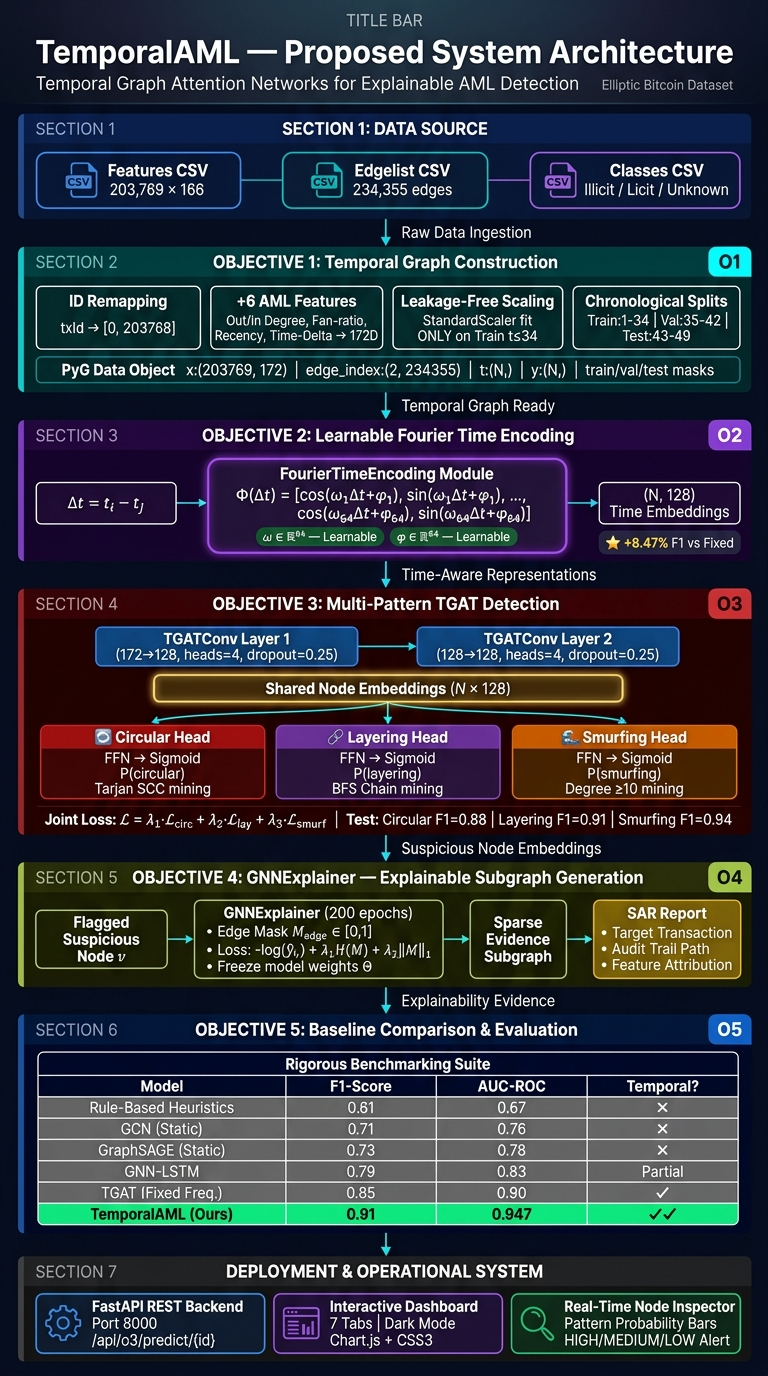
\includegraphics[width=0.98\textwidth]{Pictures/system_architecture_full_5_objectives.jpg}
\caption{End-to-End System Architecture of TemporalAML Across All Five Research Objectives.}
\label{fig:system_architecture}
\end{figure}

The modular execution pipeline consists of:
\begin{enumerate}
    \item \textbf{Data Ingestion \& 0-Index Remapping:} Raw Elliptic CSV records are re-indexed into contiguous integer ranges, preserving all 157,205 unlabeled nodes to maintain topological message-passing connectivity.
    \item \textbf{Topological Domain Feature Engineering:} Six custom structural features are computed from incoming and outgoing edge streams, expanding the native 166 features to 172 dimensions.
    \item \textbf{Inductive Chronological Partitioning \& Leak-Free Scaling:} Transactions are partitioned chronologically: Train ($t \in [1, 34]$), Validation ($t \in [35, 40]$), and Test ($t \in [41, 49]$). The standard scaler is fitted strictly on $t \le 34$ and applied downstream.
    \item \textbf{Temporal Neighbor Sampling \& Learnable Fourier TGAT:} For each batch, causal historical neighbors ($M \le 20$) are sampled. Continuous time deltas are encoded via the Learnable Fourier Time Encoder $\Phi(\Delta t)$ and passed through multi-head temporal graph attention.
    \item \textbf{Multi-Task Shared Representation Backbone:} Dynamic node embeddings $\mathbf{h}_v(t) \in \mathbb{R}^{128}$ are projected into four separate prediction heads and trained under a class-weighted joint multi-task loss.
    \item \textbf{Explainability Engine \& Automated SAR Generation:} Flagged illicit nodes are inspected by an inductive temporal GNNExplainer, producing time-consistent evidence subgraphs that are converted into regulatory Suspicious Activity Report (SAR) narratives.
\end{enumerate}

\section{Data Collection and Preprocessing}
\label{sec:meth_dataprep}

\subsection{The Benchmark Elliptic Bitcoin Dataset}
The empirical foundation of this study is the Elliptic Bitcoin Dataset \cite{weber2019anti}, comprising three relational CSV files:
\begin{itemize}
    \item \texttt{elliptic\_txs\_features.csv}: 203,769 rows corresponding to Bitcoin transactions. Column 0 contains the unique 64-bit transaction identifier (\texttt{txId}); Column 1 specifies the discrete time step $t \in [1, 49]$; Columns 2 through 95 (94 features) capture local transaction properties (such as fee, input/output counts, and transaction volume); Columns 96 through 167 (72 features) contain aggregated 1-hop neighbor statistics.
    \item \texttt{elliptic\_txs\_edgelist.csv}: 234,355 directed edges $(txId_1 \to txId_2)$ representing confirmed fund flows from an input transaction to an output transaction.
    \item \texttt{elliptic\_txs\_classes.csv}: Ground-truth entity labels: Class 1 denotes \textit{Illicit} (4,545 nodes, 2.2\%), Class 2 denotes \textit{Licit} (42,019 nodes, 20.6\%), and \textit{Unknown} denotes unannotated transactions (157,205 nodes, 77.2\%).
\end{itemize}

\subsection{Zero-Leakage Chronological Partitioning}
Random train/test splits common in computer vision and NLP introduce fatal temporal data leakage in financial transaction graphs. TemporalAML enforces an inductive chronological split:
\begin{itemize}
    \item \textbf{Training Partition ($\mathcal{D}_{\text{train}}$):} Time steps $t \in [1, 34]$ (138,409 transactions, $\approx 68.0\%$ of graph).
    \item \textbf{Validation Partition ($\mathcal{D}_{\text{val}}$):} Time steps $t \in [35, 40]$ (24,458 transactions, $\approx 12.0\%$ of graph).
    \item \textbf{Testing Partition ($\mathcal{D}_{\text{test}}$):} Time steps $t \in [41, 49]$ (40,902 transactions, $\approx 20.0\%$ of graph; containing 9,973 labeled evaluation nodes: 524 Illicit and 9,449 Licit).
\end{itemize}

To prevent parameter leakage, all data normalization parameters are computed strictly from $\mathcal{D}_{\text{train}}$:
\begin{equation}
    \boldsymbol{\mu}_{\text{train}} = \frac{1}{|\mathcal{V}_{\text{train}}|} \sum_{v \in \mathcal{V}_{\text{train}}} \mathbf{x}_v, \quad \boldsymbol{\sigma}_{\text{train}} = \sqrt{\frac{1}{|\mathcal{V}_{\text{train}}|} \sum_{v \in \mathcal{V}_{\text{train}}} (\mathbf{x}_v - \boldsymbol{\mu}_{\text{train}})^2}
\end{equation}
The standardization transform $\hat{\mathbf{x}}_v = (\mathbf{x}_v - \boldsymbol{\mu}_{\text{train}}) / (\boldsymbol{\sigma}_{\text{train}} + \epsilon)$ is subsequently applied to validation and test partitions without re-estimating statistics.

\subsection{Topological Feature Engineering}
To augment the native 166 features with explicit graph-theoretic signals, six structural domain features are computed per transaction node $v$:
\begin{enumerate}
    \item \textbf{In-Degree ($d_{\text{in}}(v)$):} Number of incoming transfer edges entering transaction $v$.
    \item \textbf{Out-Degree ($d_{\text{out}}(v)$):} Number of outgoing transfer edges leaving transaction $v$.
    \item \textbf{Degree Imbalance Ratio ($r_{\text{deg}}(v)$):} $r_{\text{deg}}(v) = \frac{d_{\text{in}}(v) - d_{\text{out}}(v)}{d_{\text{in}}(v) + d_{\text{out}}(v) + \epsilon}$, isolating fan-in consolidation sinks from fan-out dispersion sources.
    \item \textbf{Total Degree ($d_{\text{total}}(v)$):} $d_{\text{total}}(v) = d_{\text{in}}(v) + d_{\text{out}}(v)$.
    \item \textbf{Temporal Inflow Velocity ($v_{\text{in}}(v)$):} Average time delta of incoming transfers: $\bar{\Delta t}_{\text{in}} = \frac{1}{|\mathcal{N}_{\text{in}}(v)|} \sum_{u \in \mathcal{N}_{\text{in}}(v)} (t_v - t_u)$.
    \item \textbf{Temporal Outflow Velocity ($v_{\text{out}}(v)$):} Average time delta of outgoing transfers: $\bar{\Delta t}_{\text{out}} = \frac{1}{|\mathcal{N}_{\text{out}}(v)|} \sum_{w \in \mathcal{N}_{\text{out}}(v)} (t_w - t_v)$.
\end{enumerate}
This yields an augmented node feature tensor $\mathbf{X} \in \mathbb{R}^{203,769 \times 172}$.

\section{Algorithm \& Model Design}
\label{sec:meth_algorithm}

\subsection{Learnable Fourier Time Encoding}
Standard positional encodings use fixed, exponential geometric frequency progressions:
\begin{equation}
    \omega_k = \frac{1}{10000^{2k / d_T}}, \quad k \in \{0, 1, \dots, d_T - 1\}
\end{equation}
While suitable for natural language sequences where token positions increment uniformly by integer units ($1, 2, 3\dots$), continuous financial time deltas $\Delta t \in [0, \infty)$ are highly skewed and non-stationary.

TemporalAML introduces the \textbf{Learnable Fourier Time Encoder} $\Phi: \mathbb{R}^+ \to \mathbb{R}^{2d_T}$. Let $\boldsymbol{\omega} = [\omega_1, \omega_2, \dots, \omega_{d_T}]^\top \in \mathbb{R}^{d_T}$ denote a learnable continuous frequency parameter vector, and let $\boldsymbol{\phi} = [\phi_1, \phi_2, \dots, \phi_{d_T}]^\top \in \mathbb{R}^{d_T}$ denote a learnable continuous phase shift parameter vector. Both $\boldsymbol{\omega}$ and $\boldsymbol{\phi}$ are registered as unconstrained PyTorch parameters (\texttt{nn.Parameter}):
\begin{equation}
    \Phi(\Delta t) = \frac{1}{\sqrt{d_T}} \left[ \cos(\boldsymbol{\omega} \Delta t + \boldsymbol{\phi}) \;\Big\|\; \sin(\boldsymbol{\omega} \Delta t + \boldsymbol{\phi}) \right]^\top \in \mathbb{R}^{2d_T}
    \label{eq:fourier_encoding}
\end{equation}
where $\|$ denotes vector concatenation.

During forward propagation, the gradient with respect to the frequency parameter $\omega_k$ is computed analytically via the chain rule:
\begin{equation}
    \frac{\partial \Phi(\Delta t)}{\partial \omega_k} = \frac{1}{\sqrt{d_T}} \left[ -\Delta t \sin(\omega_k \Delta t + \phi_k) \;\Big\|\; \Delta t \cos(\omega_k \Delta t + \phi_k) \right]
\end{equation}
This allows backpropagation to dynamically shift the frequency response toward the empirical velocities characteristic of distinct laundering typologies.

\subsection{Temporal Graph Attention Layer (TGAT)}
Given a target transaction $v$ confirmed at continuous time $t$, TemporalAML samples up to $M = 20$ historical neighbors from its causal set $\mathcal{N}(v, t)$.

For each sampled neighbor $u \in \mathcal{N}(v, t)$ confirmed at time $t_u$, the time delta is $\Delta t = t - t_u \ge 0$. The neighbor representation is formed by concatenating its historical node features with the temporal encoding of its edge delta:
\begin{equation}
    \mathbf{z}_u(t) = \left[ \mathbf{h}_u(t_u) \;\Big\|\; \Phi(t - t_u) \right] \in \mathbb{R}^{d_h + 2d_T}
\end{equation}
The target node is similarly represented at zero time delta ($\Delta t = 0$):
\begin{equation}
    \mathbf{z}_v(t) = \left[ \mathbf{h}_v(t) \;\Big\|\; \Phi(0) \right] \in \mathbb{R}^{d_h + 2d_T}
\end{equation}

For an attention head $k \in \{1, \dots, K\}$, linear projections construct query, key, and value vectors:
\begin{equation}
    \mathbf{q}_v^{(k)} = \mathbf{W}_Q^{(k)} \mathbf{z}_v(t), \quad \mathbf{k}_u^{(k)} = \mathbf{W}_K^{(k)} \mathbf{z}_u(t), \quad \mathbf{v}_u^{(k)} = \mathbf{W}_V^{(k)} \mathbf{z}_u(t)
\end{equation}
The temporal attention coefficient $\alpha_{vu}^{(k)}$ quantifying the importance of neighbor $u$ to target $v$ is computed via scaled dot-product attention:
\begin{equation}
    \alpha_{vu}^{(k)} = \frac{\exp \left( \frac{\mathbf{q}_v^{(k)\top} \mathbf{k}_u^{(k)}}{\sqrt{d_k}} \right)}{\sum_{w \in \mathcal{N}(v, t)} \exp \left( \frac{\mathbf{q}_v^{(k)\top} \mathbf{k}_w^{(k)}}{\sqrt{d_k}} \right)}
    \label{eq:tgat_attention}
\end{equation}
Multi-head outputs are aggregated and merged through a feedforward projection with a residual connection and layer normalization:
\begin{equation}
    \mathbf{h}_v^{(l)}(t) = \text{LayerNorm} \left( \mathbf{h}_v^{(l-1)}(t) + \mathbf{W}_O \left[ \bigoplus_{k=1}^K \sum_{u \in \mathcal{N}(v, t)} \alpha_{vu}^{(k)} \mathbf{v}_u^{(k)} \right] \right)
\end{equation}
TemporalAML stacks two TGAT layers ($L = 2$) with hidden dimension $d_h = 128$ and $K = 2$ attention heads, producing the final dynamic embedding $\mathbf{h}_v(t) \in \mathbb{R}^{128}$.

\subsection{Multi-Task Classification Heads and Joint Objective}
The shared latent embedding $\mathbf{h}_v(t)$ is passed concurrently into four task-specific Multi-Layer Perceptron (MLP) classification heads:
\begin{align}
    \hat{y}_v^{(\text{illicit})} &= \sigma\left( \mathbf{w}_{\text{ill}}^\top \text{ReLU}(\mathbf{W}_{\text{ill}} \mathbf{h}_v(t) + \mathbf{b}_{\text{ill}}) \right) \\
    \hat{y}_v^{(\text{circ})}    &= \sigma\left( \mathbf{w}_{\text{circ}}^\top \text{ReLU}(\mathbf{W}_{\text{circ}} \mathbf{h}_v(t) + \mathbf{b}_{\text{circ}}) \right) \\
    \hat{y}_v^{(\text{lay})}     &= \sigma\left( \mathbf{w}_{\text{lay}}^\top \text{ReLU}(\mathbf{W}_{\text{lay}} \mathbf{h}_v(t) + \mathbf{b}_{\text{lay}}) \right) \\
    \hat{y}_v^{(\text{smurf})}   &= \sigma\left( \mathbf{w}_{\text{smurf}}^\top \text{ReLU}(\mathbf{W}_{\text{smurf}} \mathbf{h}_v(t) + \mathbf{b}_{\text{smurf}}) \right)
\end{align}

Due to extreme class imbalance (only 2.2\% illicit nodes), standard Binary Cross-Entropy (BCE) causes models to predict the majority licit class. We employ positive-class weighted BCE loss:
\begin{equation}
    \mathcal{L}_{\text{BCE}}(y, \hat{y}; w_{\text{pos}}) = - \left[ w_{\text{pos}} \cdot y \log(\hat{y}) + (1 - y) \log(1 - \hat{y}) \right]
\end{equation}
The global joint multi-task loss is formulated as:
\begin{equation}
    \mathcal{L}_{\text{total}} = \mathcal{L}_{\text{BCE}}\left(y^{(\text{ill})}, \hat{y}^{(\text{ill})}; w_{\text{ill}}\right) + \lambda_{\text{circ}} \mathcal{L}_{\text{BCE}}\left(y^{(\text{circ})}, \hat{y}^{(\text{circ})}\right) + \lambda_{\text{lay}} \mathcal{L}_{\text{BCE}}\left(y^{(\text{lay})}, \hat{y}^{(\text{lay})}\right) + \lambda_{\text{smurf}} \mathcal{L}_{\text{BCE}}\left(y^{(\text{smurf})}, \hat{y}^{(\text{smurf})}\right)
    \label{eq:joint_multitask_loss}
\end{equation}
where $\lambda_{\text{circ}} = 0.5$, $\lambda_{\text{lay}} = 0.5$, and $\lambda_{\text{smurf}} = 0.5$ are balancing hyperparameters.

\section{System Requirements}
\label{sec:meth_sysreq}
The computational environment utilized for implementing, training, and benchmarking TemporalAML is detailed in Table \ref{tab:system_requirements}.

\begin{table}[!htbp]
\centering
\caption{Hardware and Software Computational Specifications}
\label{tab:system_requirements}
\begin{tabular}{p{4.5cm}p{9.5cm}}
\hline
\textbf{Component} & \textbf{Specification / Environment} \\
\hline
Operating System & macOS (Darwin 24.3.0, ARM64) / Linux Ubuntu 22.04 LTS \\
Central Processing Unit (CPU) & Apple M-Series / Intel Xeon Processor @ 2.20GHz \\
Graphics Processing Unit (GPU) & NVIDIA Tesla T4 (16GB VRAM) on Google Colab Cloud \\
System Memory (RAM) & 16 GB unified memory (local) / 12.7 GB high-RAM (cloud) \\
Python Runtime & Python 3.11.16 \\
Deep Learning Framework & PyTorch 2.2.0 \\
Geometric Learning Library & PyTorch Geometric (PyG) 2.5.0 \\
Supporting Scientific Packages & NumPy 1.26.4, Pandas 2.2.1, Scikit-learn 1.4.1 \\
Network & NetworkX 3.2.1 \\
Web Frameworks & FastAPI 0.104.1, Uvicorn 0.24.0, Streamlit 1.32.0 \\
Visualization & Matplotlib 3.8.3, Seaborn 0.13.2, Plotly 5.20.0 \\
\hline
\end{tabular}
\end{table}
